% !TeX root = 191114.tex
\begin{frame}[t]{Книжка про Git}
Pro Git, второе издание:
\begin{center}
\href{https://git-scm.com/book/ru/v2/}{git-scm.com/book/ru/v2}
\end{center}
\end{frame}

\begin{frame}[t]{Git vs SVN}
\begin{itemize}
\item SVN "--- типичная \textit{централизованная} система: один сервер, на котором хранится вся история (SVN), локально только текущая.
	\begin{itemize}
	\item История может быть большой.
	\item Для работы нужно подключение к серверу.
	\item Можно сделать сквозную нумерацию коммитов
	\end{itemize}
\item Git "--- типичная \textit{децентрализованная} система: на каждом отдельном компьютере хранится вся история.
	\begin{itemize}
	\item Синхронизация через специальный условно-центральный компьютер.
	\item История должна помещаться на компьютер.
	\item Можно работать без сервера вообще.
	\item Генерировать номера коммитов сложно.
	\end{itemize}
\end{itemize}
	Другие особенности:
\begin{itemize}
\item В Git всё \textit{очень} хорошо с \textit{ветками}, их удобно и просто делать
\item Git сейчас модный: хостинги, инструменты, интеграции...
\item Следствие: Git проще начать пользоваться
\end{itemize}
\end{frame}

\begin{frame}[t]{Распределённые системы контроля версий}
\begin{center}
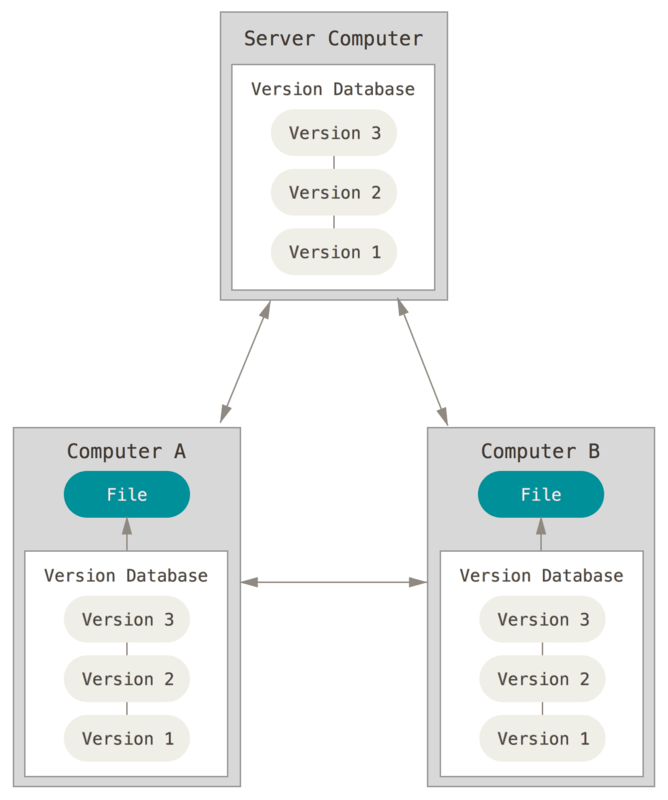
\includegraphics[height=0.8\textheight,keepaspectratio]{distributed.png}
\end{center}
\end{frame}

\begin{frame}[t]{Git vs GitHub}
Git:
\begin{itemize}
\item Система контроля версий.
\item Консольный клиент.
\end{itemize}
GitHub:
\begin{itemize}
\item Хостинг для git-репозиториев.
\item Добавляет \textit{pull requests}.
\item Добавляет \textit{интерфейс} для code review.
\item Даёт <<из коробки>> интеграции с другими инструментами.
\end{itemize}
Можно пользоваться Git без GitHub, это нормально.
\end{frame}

\begin{frame}[t]{Модель данных Git}
\begin{itemize}
\item Каждый \textit{commit} "--- отдельная версия.
\item У коммита есть \textit{предыдущий} (или несколько) "--- \textit{parent}.
\item Получаем ацикличный граф (демо ungit!)
\item \textit{Branch} (ветка) "--- указатель на комммит, двигается.
\item \textit{Tag} (тэг) "--- указатель на коммит, не двигается.
\item \textit{Remote} "--- другой репозиторий, с которым
	можно синхронизироваться (на другом компьютере).
\end{itemize}
Тонкости:
\begin{itemize}
\item Отслеживаются только файлы, не папки.
\item Отслеживается только содержимое файлов (переименование..?).
\item Никак не проверить автора или время коммита.
\item Имя коммита "--- хэш от содержимого.
\item Синхронизация "--- просто скачали себе данные в \verb~remote/ветка~,
	ветки и история локально не меняются.
\end{itemize}
\end{frame}

\begin{frame}[t]{Состояние репозитория в Git}
\begin{center}
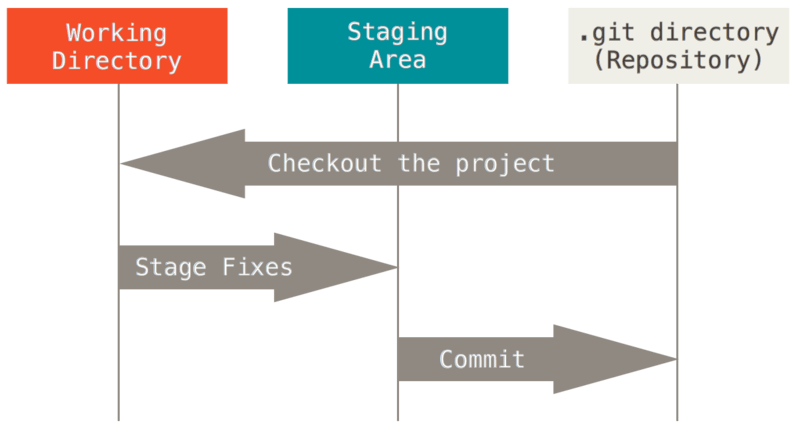
\includegraphics[width=\textwidth,keepaspectratio]{areas.png}
\end{center}
\end{frame}

\begin{frame}[t]{Состояния файлов}
\verb~git status~
\begin{center}
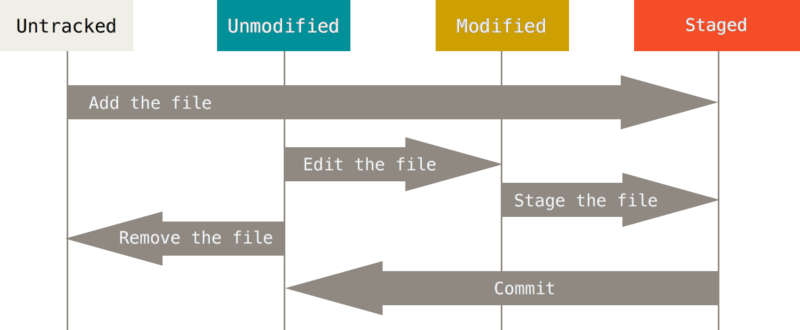
\includegraphics[width=\textwidth,keepaspectratio]{lifecycle.png}
\end{center}
\begin{itemize}
\item Ещё есть \textit{игнорирование}, оно влияет, если файл \textit{untracked}.
\item Файл может быть и \textit{modified}, и \textit{staged}.
\end{itemize}
\end{frame}

\begin{frame}[t]{Слияние веток}
\begin{center}
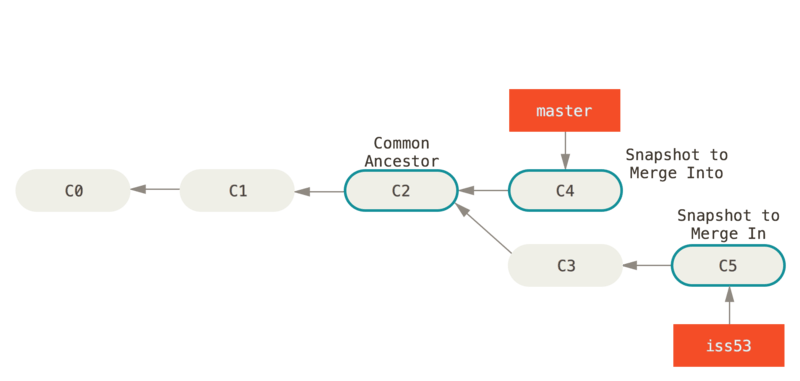
\includegraphics[width=\textwidth,keepaspectratio]{basic-merging-1.png}
\end{center}
\begin{itemize}
\item Git попытается автоматически догадаться, как склеить изменения.
\item Иногда (редко) догадывается неверно.
\item Гораздо чаще случаются \textit{конфликты} в одном файле.
\end{itemize}
\end{frame}

\begin{frame}[t]{Несколько remote}
Например, оригинальный репозиторий (upstream) и ваш форк (origin)
\begin{enumerate}
\item Подтянули изменения из upstream и origin
\item Поставили локальную ветку на ветку из origin
\item Добавили в локальную ветку изменения из upstream
\item Обновили ветку на origin
\end{enumerate}
Напрямую обновить origin из upstream нельзя!
\end{frame}
